\documentclass{beamer}
\usepackage[utf8]{inputenc}

% code snippets
\usepackage{minted}
\newmintedfile[dockercode]{dockerfile}{
  % bgcolor=mintedbackground,
  fontfamily=tt,
  linenos=true,
  numberblanklines=true,
  numbersep=5pt,
  gobble=0,
  frame=leftline,
  framerule=0.4pt,
  framesep=2mm,
  funcnamehighlighting=true,
  tabsize=4,
  obeytabs=false,
  mathescape=false
  samepage=false, %with this setting you can force the list to appear on the same page
  showspaces=false,
  showtabs =false,
  texcl=false,
}
\newminted[bashcode]{bash}{
  % bgcolor=mintedbackground,
  fontfamily=tt,
  linenos=true,
  numberblanklines=true,
  numbersep=5pt,
  gobble=0,
  frame=leftline,
  framerule=0.4pt,
  framesep=2mm,
  funcnamehighlighting=true,
  tabsize=4,
  obeytabs=false,
  mathescape=false
  samepage=false, %with this setting you can force the list to appear on the same page
  showspaces=false,
  showtabs =false,
  texcl=false,
}

% biblatex (requires biber; sudo pacman -S biber)
\usepackage[]{biblatex} % biblatex
\addbibresource{"./content/bib/bib1.bib"}
\addbibresource{"./content/bib/bib2.bib"}
\addbibresource{"./content/bib/throwaway.bib"}

\usepackage{graphicx}
\graphicspath{ {./content/img/} }

\usetheme{Boadilla}
\usecolortheme{rose}
% \beamerdefaultoverlayspecification{<+->} % this will turn it into slides

\title{Dockerisation}
\subtitle{Container technologies, for ease of development and deployment}
\author{George Onoufriou}
\date{\today}

\begin{document}

  \frame{\titlepage}

  \begin{frame}
    \frametitle{The Problem}
    \begin{itemize}
        \item You write monolithic software (lets say a whole web-stack) on machine A
        \item You test this web-stack on machine A, everything is working fine
        \item You deploy software on machine B (lets say a lab machine), oh no it doesn't have x, y, z installed
        \item You install x, y, z, but on machine A; x was version 1.2, y was version 0.0.1, z was version 1.r23345 so you go through manually install those versions
        \item web-stack still does not work properly as there was an undocumented dependency U, that you never noticed since you were always running on machine A
        \item You break down and question if you know what you are doing, as you struggle to meet a deadline
        \item You pray it works on machine C which it will be evaluated on for an assignment, it doesn't but you proclaim "it worked on my machine"
    \end{itemize}
  \end{frame}

  \begin{frame}
    \begin{figure}[th!]
      \centering
      \includegraphics[width=0.5\textwidth]{docker-is-born-meme.jpg}
      \caption{Docker is born meme.}
      \label{fig:docker_born}
    \end{figure}
  \end{frame}

  \begin{frame}
    \frametitle{How This Worked in Industry}
    \begin{figure}[th!]
      \centering
      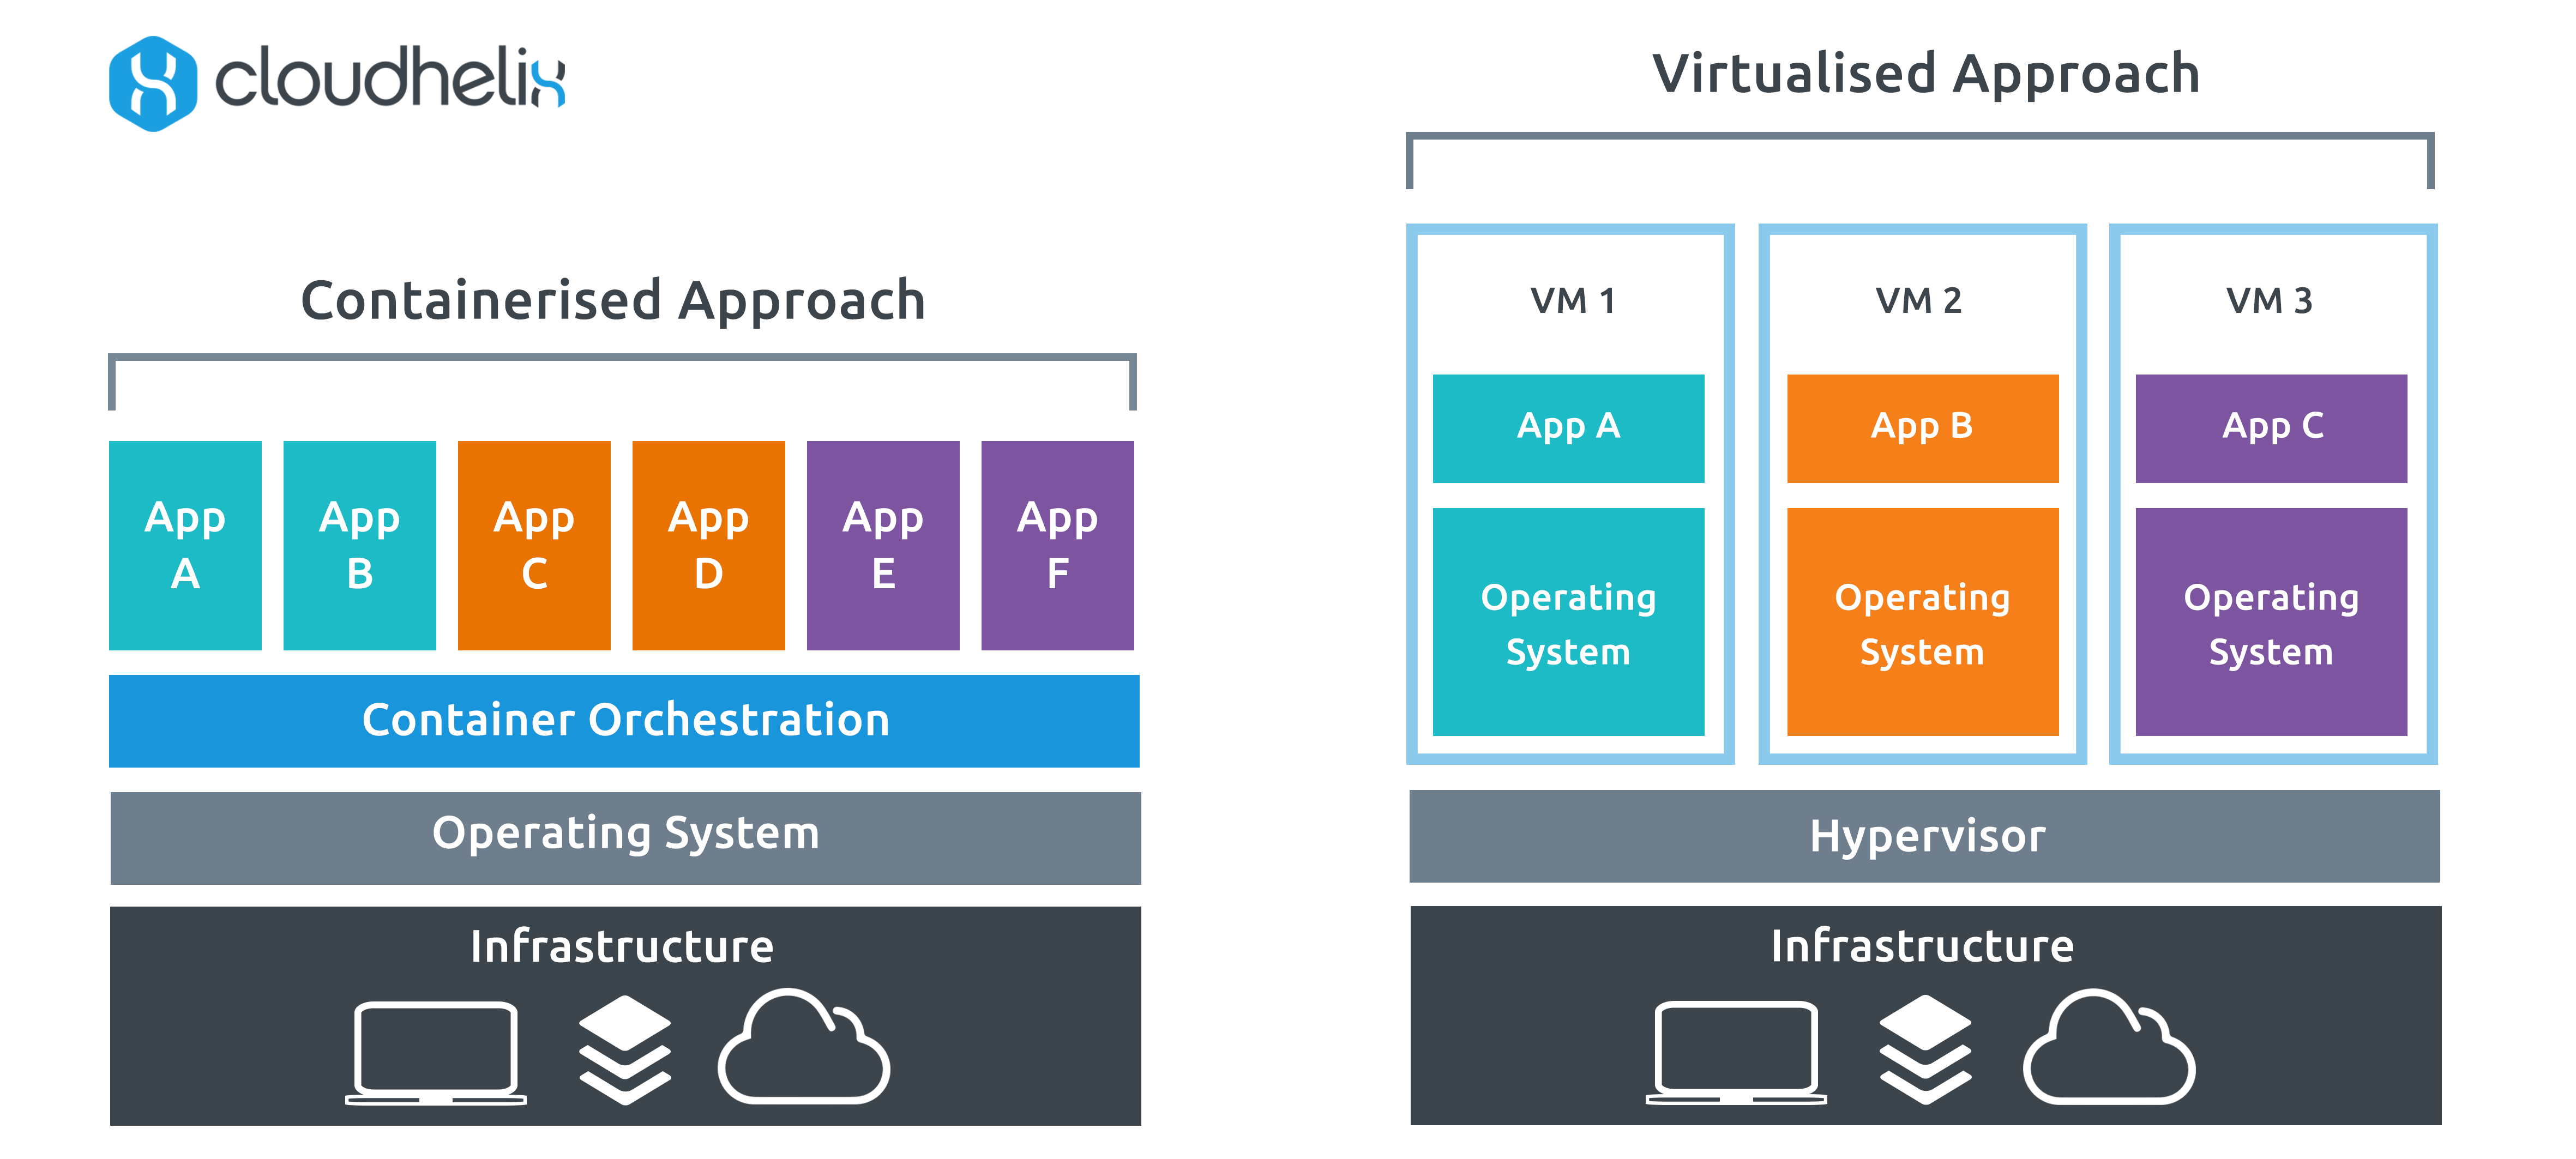
\includegraphics[width=0.9\textwidth]{containerisation.png}
      \caption{Comparing Virtualisation and Containerisation.}
      \label{fig:containerisation}
    \end{figure}
  \end{frame}

  \begin{frame}
    \frametitle{Containerisation Use Cases}
    \begin{figure}[th!]
      \centering
      
\includegraphics[width=0.4\textwidth]{kube_case_studies.png}
      \caption{Sample Kubernetes use in the wild. \autocite{kube_cases}}
      \label{fig:kube_use}
    \end{figure}
  \end{frame}

  \begin{frame}
    \frametitle{What is Docker}
    \begin{itemize}
        \item Repeatable instructions to (re)create a lightweight virtual machine
    \end{itemize}
    \begin{figure}[th!]
      \centering
      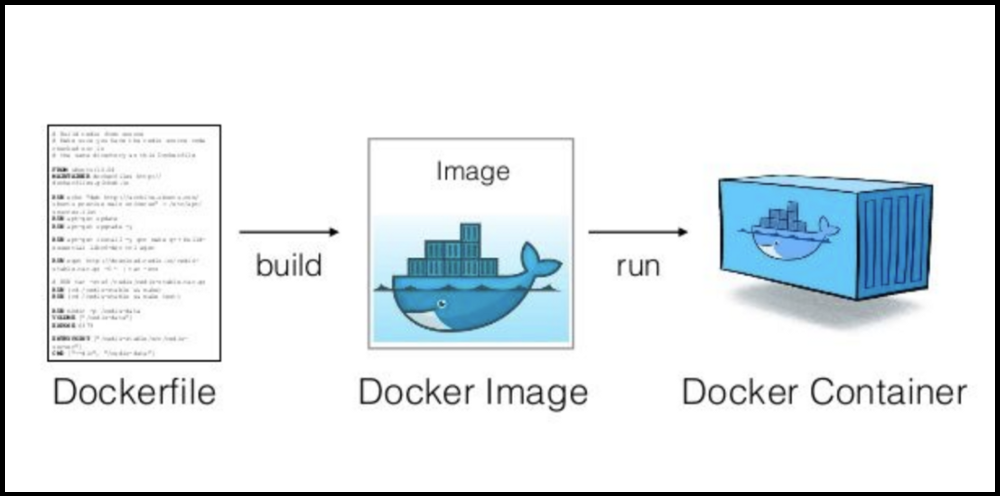
\includegraphics[width=0.7\textwidth]{docker_process.png}
      \caption{Creating Docker Containers. \autocite{docker_build}}
      \label{fig:docker_build}
    \end{figure}
  \end{frame}

  \begin{frame}[fragile]
    \frametitle{Dockerfile build}
    % \inputminted{dockerfile}{content/src/Dockerfile}
    \textbf{\textit{./Dockerfile}}:
    \dockercode{content/src/Dockerfile}
    to build this file (-f Dockerfile) located in this directory ('.') and tag it with name: \textit{"some/tag"}:
    \begin{bashcode}
docker build -t some/tag -f Dockerfile .
    \end{bashcode}
  \end{frame}

  \begin{frame}
    \frametitle{Dockerfile Build This Presentation}
    \textbf{\textit{./Dockerfile}}:
    \dockercode{Dockerfile}
  \end{frame}

  \begin{frame}[fragile]% FRAGILE REQUIRED FOR BEAMER + MINTED TO WORK
    \frametitle{Docker Image Use}
    \begin{itemize}
        \item Build a "Dockerfile" file and  tag it as "some/tag":
        \begin{bashcode}
docker build -t some/tag -f Dockerfile .
        \end{bashcode}
        \item Run bash from inside this image known as "some/tag" interactively:
        \begin{bashcode}
docker run -it some/tag bash
        \end{bashcode}
        \item Same as above but now with gpu passthrough and directly calling nvidia-smi to view them
        \begin{bashcode}
docker run --gpus all -it some/tag nvidia-smi
        \end{bashcode}
    \end{itemize}
  \end{frame}

  \begin{frame}
    \frametitle{Docker Zero to Dev}
    \begin{itemize}
      \item Docker (single container)
      \item Docker-Compose (single node container orchestrator)
      \item Docker Swarm (or other multi node container orchestrator)
    \end{itemize}
    \begin{itemize}
      \item Kubernetes
      \item Apache Mesos
    \end{itemize}
  \end{frame}

  \begin{frame}
    \frametitle{Docker-Compose}
  \end{frame}

  \begin{frame}[allowframebreaks]
    \frametitle{References}
    % % biblatex version
    \printbibliography
  \end{frame}

\end{document}
